\documentclass{article}

\usepackage{coursenotes}

\set{AuthorName}{TC Fraser}
\set{Email}{tcfraser@tcfraser.com}
\set{Website}{www.tcfraser.com}
\set{ClassName}{General Relativity}
\set{School}{University of Waterloo}
\set{CourseCode}{Phys 476}
\set{InstructorName}{Florian Girelli}
\set{Term}{Winter 2016}

\begin{document}

\titlePage

\tableOfContents

\disclaimer


\section{Introduction}

\subsection{History}

The first lecture was a summary of astrophsyical history from around $\sim$200BC to today. I elected not to take notes as it was pretty standard stuff and a lot of slides. Sorry.

\section{Tensor Formalism}

At the core of General Relativity is the mathematics of differential geometry. Differential geometry requires the idea of tensors, a generalization of vectors and matricies and forms that can handle messy geometries and metrics. \\

Let $V$ be a vector space of finite dimension. Any $V$ is isomorphic to $\R^{n+1}$ through the coefficients of a chosen basis. Let the basis of $V$ be given by,

\[ \bc{e_i}_{i=\tok0n} \]

Then any vector $v \in V$ is expressible by,

\[ v = \sum_{i=0}^{n} v^i e_i \]

Where $v^i$ are the $i$-th coefficients of the vector $v$ with respect to the basis $\bc{e_i}$.

\subsection{Einstein Summation Rule}

For convience let's provide a new, shorter notation for the vector $v$.

\[ v^ie_i = v^0e_0 + \ldots + v^ne_n = \sum_{i=0}^nv^ie_i \]

Effectively, we have just \textbf{dropped the summation sign}. The einstein summation rule is as follows: \\

If there are two identical indicies, 1 ``up'' and 1 ``down'', it means that a summation is secretly present, it's just be removed for convience. Note that the $i$ in this case is \textit{dummy index}.

\[ v^ie_i = v^{\alpha}e_{\alpha} = v^je_j \]

Here $v^i$ are the components of vector $v \in V$ and are real numbers. $v^i \in \R, \forall i \in \bc{\tok0n}$. \\

Note $v^i$ is called the vector $v$ when $i$ is the set $\bc{\tok0n}$, but can also be called the $i$-th component of $v$ when $i$ has a fixed value $i \in \bc{\tok0n}$. \\

\subsection{Examples of Basis for V}

The values of $e_i$ or the $i$'s themselves can take on many possible values.

\begin{itemize}
    \item cartesian coordinates $t,x,y,z$
    \item spherical coordinates $t, r, \phi, \theta$
    \item etc.
\end{itemize}

Each of the above examples is the space $V = \R^4$ (with some bounds for spherical coordinates).

\subsection{Dual Vector Space}

The dual vector space of $V$ denoted $V^*$ is also isomorphic to $\R^{n+1}$ and is built from the space of linear forms on V.

\[ V^* = \bc{w: V \ar \R \st w(\alpha v_1 + \beta v_2) = \alpha w( v_1) + \beta w(v_2)} \]

where $v_1, v_2 \in V$ and $\alpha, \beta \in \R$.

In Quantum Mechanics, the vectors are the bras and the elements of the dual space (called the covectors) are the kets. \\

We note,

\[ \bc{f^i}_{i=\tok0n} \]

is the basis for $V^*$ is defined by the kronecker symbol $\delta$,

\[ f^j(e_j) = {\delta^j}_i \]

\[ {\delta^j}_i = \piecewise{1}{i=j}{0}{i\neq j} \]

An element in $V^*$ is $w = w_if^i$. $w_i$ are the components of the covector $w$. Note that for a \textbf{finite dimensional vector space},

\[ V^{**} = V \]

\subsection{Bilinear Maps}

Introduce a bilinear map $B(v, w)$ where $B: V \cross V \ar \R$ where,

\[ B(\alpha v_1 + \beta v_2, w) = \alpha B(v_1, w) + \beta B(v_2, w) \]

and the same for the other parameter $w$. \\

Examples include the inner product (otherwise known as the scale or dot product).

Bilinear forms are bilinear maps such that the following conditions are true:

\begin{itemize}
    \item symmetric: $B(v,w) = B(w,v)$
    \item non-degenerated: $B(v,w) = 0 \quad \forall v \implies w = 0$
\end{itemize}

Playing with indicies,

\begin{align*}
    B(v,w) &= B(v^\alpha e_\alpha, w^\beta e_\beta) \\
           &= v^\alpha B( e_\alpha, w^\beta e_\beta) \note{By linearity} \\
           &= v^\alpha w^\beta B( e_\alpha, e_\beta) \note{By linearity}
\end{align*}

A bilinear map used in this way provides a way to eliminate the headache of complicated cross sums. Define new notation,

\[ B( e_\alpha, e_\beta) \defined g_{\al\be} \]

Where $g_{\al\be}$ is a real number $\R$ because $\al$ and $\be$ are summed over.

\[ B(v, w) = v^\al w^\be g_{\al\be} = v^\al g_{\al\be}w^\be =  w^\be g_{\al\be} v^\al \]

All of the above terms are commutative because in the end, it represents a sum over all $\al, \be$.

\[ B(v,w) = \underbrace{v^0w^0g_{00} + \ldots + v^2w^3g_{2,3} + \ldots + v^nw^ng_{nn}}_{(n+1)^2 \text{terms}} \]

\subsection{Distance and Norms}

To define a distance in a vector space, we can use norms. In this case, $g_{\al\be}$ would be called the metric. The Euclidean metric (with respect to a cartesian basis) for example would be,

\[ g_{\al\be} = \piecewise{1}{\al = \be}{0}{\al \neq \be}  \]

We can also choose to enforce that the basis be orthonormal,

\[ B(e_i, e_j) = \piecewise{\pm1}{i = j}{0}{i \neq j} \]

Note that the potential for a negative norm means the notion of positive definiteness is no longer gauranteed.

\subsection{Signatures of Metrics}

We call the signature of the metric the number of $+1$'s and $-1$'s appearing in $g_{ij}$ when dealing with the orthonormal basis. Signature is denoted as:

\[ \br{p, q} = \br{\underbrace{p}_{\text{postive}}, \underbrace{q}_{\text{negative}}} \]

For example,

\begin{itemize}
    \item Euclidean metric: $(n+1, 0)$
    \item Minkowski metric: $(n, 1)$
\end{itemize}

Note the order of the signature is chosen to be $(p,q)$ and not $(q, p)$ by convention.

\subsection{Covectors from Vectors}

Note that $v^i$ was called the vector and $w_i$ was called the covector. This notation seems to indicate that conversion between $V$ and $V^*$ is notationally equivalent to raising and lowering the indicies. \\

We call the following opperation ``Lowering the index using the metric''.

\[ \underbrace{v^\al}_{\text{components of vector}} \mapsto g_{\al\be} v^\be = \underbrace{v_\al}_{\text{components of covector}} \]

In use,

\[ B(v,w) = v^\al g_{\al\be} w^\be = \untext{v_\be}{bra} \untext{w^\be}{ket} \]

\subsection{Linear Map on V to V}

\[ M : V \ar V \]

Where M is a matrix. An the map is equivalent to $v \ar Mv \in V$. Some definition,

\[ \br{Mv}^\al = \untext{{M^\al}_\be}{Matrix \\ (components)} v^\be \]

Note that ${M^\al}_\be \in \R$ for $\al$ and $\be$ fixed. Example: The identity matrix is denoted ${\delta^\al}_\be = \mathbb{I}$.

\subsection{Scalar Product on Dual Space}

Introduce a scalar product for the covectors $w$.

\[ w, t \in V^* \]

\[ w \cdot t = w_\al h^{\al\be} t_\be \]

Where $h^{\al\be}$ is symmetric and non-degenerate.

So how is the scalar product between the dual and normal space related? Specifically how are $g_{\al\be}$ and $h^{\al\be}$ connected? Well,

\begin{align*}
   v^\al g_{\al\be} w^\be &= v^\al w_\al \\
   &= v_\ga h^{\ga\al} w_\al \\
   &= v^\nu g_{\nu\ga} h^{\ga\al} w_\al \\
   &= v^\nu g_{\nu\ga} h^{\ga\al} g_{\al\mu} w^\mu
\end{align*}

Since this is true for any $v$ and $w$ we require that,

\[ h^{\ga\al} g_{\al\mu} = {\delta^\ga}_\mu \]

This means we say that the metric $h$ is the inverse of the metric $g$. Convention on $V^*$: we denote the metric $g^{\al\be}$ (the indicies are ``up''). \\

\subsection{Invariance of Scalar Product}

Let us say we have a matrix $M : v \ar \ti{v} = Mv, w \ar \ti{w} = Mw$ and that $M$ preserves the scalar product.

\[ \ti{v} \cdot \ti{w} = v \cdot w \qquad \forall v, w \]

Examine,

\[ {M^\ga}_\al v^\al g_{\al\be} {M^\be}_\rho w^\rho = v^\al g_{\al\be}w^\be \]

Use communitivity and dummyness of indicies to obtain,

\[ v^\al {M^\ga}_\al g_{\al\rho} {M^\rho}_\be w^\be = v^\al g_{\al\be}w^\be \]

Drop outer covectors $v$ and $w$ to get,

\[ {M^\ga}_\al g_{\al\rho} {M^\rho}_\be = g_{\al\be} \numberthis \label{eq:invarM} \]

Note that this expression is consistent with the Einstein summation convention. \\

An example of an $M$ on euclidean space could be a rotation matrix, or the identity. \\

When $M$ satisfies \ref{eq:invarM}, it is said to be orthogonal. It $\det(M) = 1$ then we say that $M$ is \textit{special}.

\subsection{Trace of M}

What is the trace of $M$?

\[ \Tr(M) = {M^\al}_\al = {M^0}_0 + \ldots + {M^n}_n\]

This is just a notationally convention. It is the sum of the diagonal terms of $M$.

\subsection{Tensor Product}

A tensor product makes a linear map a multi-linear map.

\heading{Theorem}

Let $E$ and $F$ be 2 vector spaces (with finite dimensionality.)

$\exists $ a unique ($!$) set (up to isomorphism) $E \otimes F$ such that if $f$ is a bilinear map $f: E \cross F \ar \R$ then $\exists$ a linear map $f^* : E \otimes F \ar \R$ such that $f = f^* \circ \phi$ with

\begin{center}
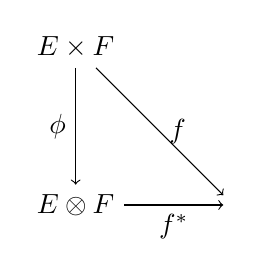
\begin{tikzpicture}
\node (EtimesF) at (0,0) {$E \times F$};
\node (EotimesF) at (0,-2) {$E \otimes F$};
\node (R) at (2,-2) {$\R$};
\draw [->] (EtimesF) edge node[left] {$\phi$} (EotimesF);
\draw [->] (EtimesF) edge node[right] {$f$} (R);
\draw [->] (EotimesF) edge node[below] {$f^*$} (R);
\end{tikzpicture}
\end{center}

Then we have,

\[ \Lin(E \otimes F, \R) \iso \Bin(E \cross F, \R) \]
\[ \Lin(f^*, \R) \iso \Bin(f, \R) \]

where `$\iso$' is used to denote \textit{isomorphic}.

\heading{Properties}

Basis for $E \otimes F$ is $e_\al \otimes g_\al$ where $e_\al$ is the basis for E and $g_\al$ is the basis for F.
For $a \in \R$ and $t, v \in E$, $u, w \in F$,

\begin{itemize}
    \item $\dim(E \otimes F) = \dim(E)\dim(F)$
    \item $a (v \otimes w) = (av) \otimes w = v \otimes (aw)$
    \item $(v + t) \otimes w = v \otimes w + t \otimes w$
    \item $v \otimes (w + u) = v \otimes w + v \otimes u$
    \item $a \otimes w = aw$
    \item $\R \otimes F = F$
\end{itemize}

Note that $V^* \otimes V^* \iso \Bin(V \times V, \R)$. To motivate this, let $f^\al \otimes f^\be$ be the basis for $V^* \otimes V^*$, and then a general element in $V^* \otimes V^*$ is,

\[ t = t_{\al\be} f^\al \otimes f^\be \]

Note that $t_{\al\be}$ is just a set of numbers. Then the tensor product is expanded as follows,

\begin{align*}
    t (v \otimes w) &= t (v^\al e_\al \otimes w^\be e_\be) \\
    &= t_{\ga\de} (f^\ga \otimes f^\de) (v^\al e_\al \otimes w^\be e_\be) \\
    &= t_{\ga\de} v^\al w^\be (f^\ga \otimes f^\de) (e_\al \otimes e_\be) \note{By linearity} \\
    &= t_{\ga\de} v^\al w^\be f^\ga(e_\al) f^\de(e_\be) \note{By foiling and definition of $f$} \\
    &= t_{\ga\de} v^\al w^\be {\delta^\ga}\al {\delta^\de}_\be \\
    &= t_{\ga\de} v^\ga w^\be {\delta^\de}_\be \note{By sifting property of $\delta$}\\
    &= t_{\ga\de} v^\ga w^\de \note{By sifting property of $\delta$ again}
\end{align*}

Since $t (v \otimes w)$ is the tensor product $V^* \otimes V^*$ and $t_{\ga\de}$ is the components of the bilinear form, one can see the connection $V^* \otimes V^* \iso \Bin(V \times V, \R)$. \\

Tensors allow one to write bilinear maps as linear maps. What about multi-linear maps?

\heading{Tensors}

A tensor of rank $\br{k,l}$ is a multilinear map

\[ \underbrace{V^* \times \cdots \times V^*}_{k} \times \underbrace{V \times \cdots \times V}_{l} \ar \R \]

which transforms \textit{well} under the change of basis of $V$ and $V^*$. \\

\begin{center}
\label{Tensor Examples}
\begin{tabular}{c|c}
Tensor & Rank \\
\hline
vectors & $(1,0)$ \\
covectors & $(0,1)$ \\
scalar & $(0,0)$ \\
metric & $(0,2)$ \\
inverse metric & $(2,0)$ \\
matrix & $(1,1)$ \\
\end{tabular}
\end{center}

The set of tensors of rank $(k,l)$ is a vector space of dimension $n^{k+l}$ (if $V$ has dimension $n$). Checking with the examples above motivates this fact. \\

Using the basis $e_{\al_1} \otimes \cdots \otimes e_{\al_k} \otimes f^{\be_1} \otimes \cdots \otimes f^{\be_k}$

\[ T = {T^{\al_1\al_2\cdots\al_k}}_{\be_1\be_2\cdots\be_l} e_{\al_1} \otimes \cdots \otimes e_{\al_k} \otimes f^{\be_1} \otimes \cdots \otimes f^{\be_k}\]

For fixed $\al_i$ and $\be_i$ this is a real number in $\R$. These are the \textit{components of the tensor}. \\

By abuse of notation we will call ${T^{\al_1\al_2\cdots\al_k}}_{\be_1\be_2\cdots\be_l}$ the tensor. \\

We are talking about these transformations as change of basis of $V$ and $V^*$. Examples:
\begin{itemize}
  \item rotations (boost)
  \item change of coordinates from cartesian to spherical, cylindrical, etc.
\end{itemize}

We can have a linear change of basis $\ti{x}^\mu = {A^\mu}_\nu x^\nu $.

\heading{Example}

\begin{center}
\begin{tabular}{c|c}
    Cartesian & Polar \\
    \hline
    $e_1 = \vec{i}$ & $\ti{e}_1 = e_r$ \\
    $e_2 = \vec{j}$ & $\ti{e}_2 = e_\theta$ \\
\end{tabular}
\end{center}

\heading{Example}

\[ \ti{e}_\al = \untext{\pder{x^\nu}{\ti{x}^\al}}{Jacobian} e_\nu = {A^{\nu}}_\al e_\nu \]

Note: \textit{Up in the denominator means down on the original coordinates (LHS).}

For example,

\begin{center}
\begin{tabular}{c|c}
    $x^1 = x$ & $\ti{x}^1 = r$ \\
    $x^2 = y$ & $\ti{x}^2 = \theta$ \\
\end{tabular}
\end{center}

\[ \ti{e}_1 = e_r = \pder{x^1}{\ti{x}^1} e_1 + \pder{x^2}{\ti{x}^1} e_2 = \cos \theta e_1 + \sin \theta e_1 \]
\[ \ti{e}_2 = e_\theta = \pder{x^1}{\ti{x}^2} e_1 + \pder{x^2}{\ti{x}^2} e_2 = - r \sin \theta e_1 + r \cos \theta e_1 \]

\heading{Vectors in multiple basis}

\[ v = v^\nu e_\nu = \ti{v}^\nu \ti{e}_\nu \]

With conversion of basis given by,

\[ \ti{e}_\al = {A^\nu}_al e_\nu\]

Thus substituting in,

\[ v^\nu e_\nu = \ti{v}^\al {A^\nu}_\al e_\nu \]

\[ v^\nu = \ti{v}^\al {A^\nu}_\al \]

But with $A$ as a Jacobian,

\[ v^\nu = \pder{x^\nu}{\ti{x}^\al} \ti{v}^\al \]
\[  \ti{v}^\al = \pder{\ti{x}^\al}{x^\nu} v^\nu \]

But what about the dual space?

By definition,

\[ \ti{f}^\be\br{\ti{e}_\nu} = \delta^\be_\mu = \ti{f}^\be \br{{A^\al}_\nu e_\al} = {A^\al}_\nu \ti{f}^\be \br{ e_\al}\]

Let $\ti{f}^\be \br{ e_\al}$ be expressed as $\ti{f}^\be = {B^\be}_\ga f^\ga$

\begin{align*}
    \ti{f}^\be\br{\ti{e}_\nu} &= {A^\al}_\nu {B^\be}_\ga f^\ga \br{ e_\al} \\
    &= {A^\al}_\nu {B^\be}_\ga {\delta^\ga}_\al \\
    &= {B^\be}_\ga {A^\ga}_\nu \\
    &= {\delta^\be}_nu
\end{align*}

Thus $B$ is the inverse of $A$. \\

What is performing \textit{well}? A tensor is performming well if it's compponents transform as

\[{T^{\nu_1\nu_2\cdots\nu_k}}_{\al_1\al_2\cdots\al_l} \ar \pder{\ti{x}^\nu_1}{x^\be_1} \cdots \pder{\ti{x}^\nu_k}{x^\be_k} \pder{x^\ga_1}{\ti{x}^\al_1} \cdots \pder{x^\ga_k}{\ti{x}^\al_k} {T^{\be_1\be_2\cdots\be_k}}_{\ga_1\ga_2\cdots\ga_l} = {\ti{T}^{\nu_1\nu_2\cdots\nu_k}}_{\al_1\al_2\cdots\al_l} \]

If you find something like ${T^\al}_\be$ is it a tensor? \textbf{No! You must check if it transforms well.}

\[ \pder{}{x^\nu} v^\al \note{This is not a tensor.} \]

The derivative here prevents it from being well-formed. In the future we will define a derivative that allows a tensor to transform well.

\subsection{Operations on Tensors}

\begin{itemize}
    \item Add (with matching rank): ${T^{\al_1\al_2}}_{\be_1\be_2} + {C^{\al_1\al_2}}_{\be_1\be_2}$.
    \item Contraction (partial trace): $\mathcal{T} (k, k) \ar \mathcal{T} (k-1, k-1)$.
    \begin{itemize}
        \item ${T^{\al_1\cdots\al_i\cdots\al_k}}_{\be_1\cdots\be_j\cdots\be_l} \ar {T^{\al_1\cdots\al_i\cdots\al_k}}_{\be_1\cdots\al_j\cdots\be_l}$
    \end{itemize}
    \item ``Outer'' Product (Gluing together tensors)
    \begin{itemize}
        \item $\mathcal{T}(k,l) \times \mathcal{T}(k',l') \ar \mathcal{T}(k + k', l+ l')$
        \item $(T_1, T_2) \ar T_1T_2$
        \item $T_1 T_2 \ar {T_1^{\nu_1\cdots\nu_k}}_{\al_1\cdots\al_l} {T_2^{\be_1\cdots\be_k}}_{\ga_1\cdots\ga_l}$
        \item \textbf{Example:} $\br{v^\al. w_\be} \ar v^\al \otimes w_\be = v^\al w_\be$. (In QM this is $\ket{\phi}\bra{\varphi}$)
    \end{itemize}
\end{itemize}

The metric $g_{\al\be}$ can change the rank of a tensor. Recall a metric is rank $(0,2)$ is symmetric and is non-degenerate.

\heading{Example}

Changing from rank $(1,0)$ to rank $(0,1)$:

\[ v^\al \ar v_a = g_{\al\be} v^\be \]

Changing from rank $(2,2)$ to rank $(4,0)$:

\[ {c^{\al\be}}_{\ga\de} \ar c_{\al\be\ga\de} = g_{\al\rho}g_{\be\eta} {c^{\rho\eta}}_{\ga\de} \]

Changing from rank $(2,2)$ to a different rank $(2,2)$:

\[ {c^{\al\be}}_{\ga\de} \ar {{{c^{\al}}_\be}^{\ga}}_\de = g_{\be\rho}g^{\ga\eta} {c^{\al\rho}}_{\eta\de} \]

\subsubsection{Facts About Tensors}

\heading{Order Matters}

\begin{align*}
{c^\al}_\be &: \qquad V^* \times V \ar \R \\
{c_\al}^\be &: \qquad V \times V^* \ar \R \\
c_\al^\be &: \qquad \text{Nothing. Don't do this.} \\
\end{align*}

\heading{Equality between tensors}

As tensors, indicies must match:\\

Position of indicies is matching: ${{c^\al}_\ga}^\de = {{T^\al}_\ga}^\de$ \\

Position of indicies is \textbf{not} matching: ${{c^\al}_\ga}^\de \neq {{T^\al}_\ga}_\de$ \\

But for fixed $\al, \ga, \de$, one can abuse the notation a bit:

\[ {{c^\al}_\ga}^\de = {{T^\al}_\ga}_\de \note{Try to avoid this.}\]

\subsection{Outer Product and Contraction}

\heading{Example}

Outer Product: ${M^{\al}}_\be{M^{\ga}}_\de = {{{{C^{\al}}_\be}^\ga}_\de}$ \\
Contraction: ${M^{\al}}_\be{M^{\be}}_\de = {{{{C^{\al}}_\be}^\be}_\de} = {C^\al}_\ga$

\heading{Example}

Outer product and contraction: ${C^{\al\be}}_{\ga\de}{T^{\ga\de}}_{\rho} = {A^{\al\be}}_\rho$ \\
This doesn't make sense: ${C^{\al\be}}_{\ga\ga}{T^{\ga\de}}_{\rho} = ??$

Note, when there is a ``+'' sign we can be ``loose'' with the indicies. Here the dual indicies \textbf{do not} indicate a summation. This acts as an abuse of notation, but is sometimes difficult to avoid.

\[ C^{\al\ga}{T_\ga}^{\de} + {F_\ga}^{\de}A^{\al\ga} \]

\subsection{Interpretation of Tensors}

By looking at the indicies, how can we interpret the physical meaning of the tensor object? \\

\begin{tabular}{c|l}
    Tensor & Interpretation \\
    \hline
    $v^\nu$ & vector \\
    $v_\nu$ & covector \\
    ${M^\al}_\be$ & matrix ($\al$ rows, $\be$ columns) \\
    ${M^\al}_\al$ & contracted matrix (trace) \\
    ${M^{\al\ga}}_\de$ & matrix whose elements are vectors themselves (${\cdot^\ga}_\de$ is the matrix) \\
    ${M^{\al\ga}}_\de$ & vector with matrix components (${M^\al}$ is the vector) \\
    ${R^{\al\be}}_{\ga\de}$ & matrix of matricies *\\
\end{tabular}
\vspace{0.1in}

*For example, if $\dim V = 4$, ${R^{\al\be}}_{\ga\de}$ has $4^4 = 256$ components. Note however, there can be many symmetries that reduce the number of unique components.

\subsection{Symmetry of Tensor}

We can always build a symmetric and antisymmetric part of a tensor $T^{\al\be}$. Let's look at the case of 2 indicies $\al, \be$:

\heading{Symmetric Part}

\[ T_{\br{\al\be}} = \f12 \br{T_{\al\be} + T_{\be\al}} \]
\[ T_{\br{\al\be}} = T_{\br{\be\al}}  \]

\heading{Antisymmetric Part}

\[ T_{\bs{\al\be}} = \f12 \br{T_{\al\be} - T_{\be\al}} \]
\[ T_{\bs{\al\be}} = - T_{\bs{\be\al}}  \]

Note that for all tensors $T^{\al\be} = T^{\br{\al\be}} + T^{\bs{\al\be}}$. This acts as the decomposition into odd and even symmetries of the tensor. \\

For more indicies:

\[ {T^{\br{\al\be}}}_{\bs{\ga\de}} = \f14\br{{T^{\al\be}}_{\ga\de} + {T^{\be\al}}_{\ga\de} - {T^{\al\be}}_{\de\ga} - {T^{\be\al}}_{\de\ga}} \]

What does $T^{\br{\al\be\ga}}$ mean? For that we will need a permutation group.

\section{Physics Review}

Moving away from tensors for a moment... \\

\subsection{Newtonian Physics}

According to Galileo and Newton, we got the interpretation that both space and time if flat $\br{\R^3}$ and is absolute. More specifically, all clocks have the same time on them if they are started at the same time. \\

Built on cartesian coordinate system: $\br{\vec{x}, t}$. With this we say that an object is at position $\vec{x}$ at time $t$. They are \textit{outcomes of measurements}. In General Relativity, the notion of coordinates can be quite different. \\

Consider a particle (2d spacetime):

\begin{center}
\begin{tikzpicture}[scale=1.0]
    % Draw axes
    \draw [<->,thick] (0,4) node (yaxis) [above] {$x$}
        |- (5,0) node (xaxis) [right] {$t$};
    \draw [blue, thick, ->] plot [smooth, tension=1] coordinates { (0,1) (1,2) (3,1) (4,3)};
    \node [blue,above] (label) at (1,2) {$x(t)$};
\end{tikzpicture}
\end{center}

Typically, $x$ is drawn as the ordinate ($y$-axis) and $t$ as the abscissa ($x$-axis).

\heading{Spacetime diagram}

In a spacetime diagram, $t$ is drawn as the ordinate.

\begin{center}
\begin{tikzpicture}[scale=1.0]
    % Draw axes
    \draw [<->,thick] (0,4) node (yaxis) [above] {$t$}
        |- (5,0) node (xaxis) [right] {$x$};
    \draw [blue, thick, ->] plot [smooth, tension=1] coordinates { (1,0) (2,1) (1,3) (3,4)};
    \node [blue, right] (label) at (2,1) {$x(t)$};
\end{tikzpicture}
\end{center}








\end{document}